\section{System Modeling}
\subsection{Source-derived multibody plant}
The original model is \texttt{ballbotgym/ballbotgym/assets/bbot.xml}. The research factory adds a cylindrical shell, mounting supports, and payload bodies to a generated model without modifying that original file. Three actuated wheel hinges are arranged at body yaw offsets of $0$, $120$, and $240$ degrees. They contact a separate spherical body. The sphere radius is $0.09$ m, and each motor has unit gear and a nominal command range of $[-10,10]$ Nm. The wheel geometry is represented with capsules and anisotropic contact parameters; it is an approximation to omnidirectional-wheel mechanics rather than a resolved roller assembly.\claim{C01}

The archived loaded model used for parameter extraction has total body mass $4.73744693$ kg. Its base body mass is $3.45119170$ kg, with principal inertia approximately $(0.03286527,0.03286527,0.02285304)$ kg m$^2$ and body-frame inertial position $(0,0,0.01641124)$ m. These are compiled simulation parameters, including geometry-derived properties, not independently measured hardware values. The evidence package records every body's mass, inertial frame, and tensor components so that a single base inertia is not mistaken for the locked inertia of the whole robot.\claim{C02}

Two free joints describe base and ball poses; three wheel hinges and two modal slides complete the loaded plant. Quaternions represent free-body orientations. The compiled model consequently has $19$ position coordinates, $17$ generalized velocities, and three motor controls. A conceptual multibody description is
\begin{equation}
 M(Q)\dot V+c(Q,V)+g(Q)=S^T\tau+J^T\lambda+f_p(Q,V),
\end{equation}
where $Q$ includes quaternion coordinates, $V$ is the velocity representation, $S$ selects actuators, $\lambda$ represents constraint/contact forces, and $f_p$ includes passive springs and damping. This summarizes native simulation, not an analytical equation explicitly solved by the cascade controller.\claim{C03}

\subsection{Implemented modal payload}
The liquid surrogate uses one moving body with two orthogonal slides. Its coordinates $q=(q_x,q_y)$ and relative velocities $v$ describe lateral generalized displacement in the tank frame. A fixed body carries the remaining liquid mass. The total mass is counted once: two slide coordinates do not imply two copies of the moving mass. For a cylindrical radius $R$, liquid volume $V_l$, density $\rho$, depth $h=V_l/(\pi R^2)$, and $\xi=1.8411837813406593$, the implementation defines
\begin{align}
 m_l&=\rho V_l,\quad \omega^2=\frac{g\xi}{R}\tanh(\xi h/R),\\
 m_1&=m_l\frac{2R\tanh(\xi h/R)}{h\xi(\xi^2-1)},\\
 m_0&=m_l-m_1,\quad k=m_1\omega^2,\quad c=2\zeta\omega m_1.
\end{align}
The nominal $0.5$ L case uses $\rho=998$ kg/m$^3$, $R=0.07$ m, and assumed $\zeta=0.02$. This gives $m_l=0.499$ kg, $m_1=0.33888497$ kg, $\omega=13.37524111$ rad/s, $k=60.62552917$ N/m, and $c=0.18130673$ Ns/m.\claim{C04}

Both liquid bodies are placed at nominal half-depth. The fixed body carries the cylindrical inertia with a small inertia allocation reserved for the moving body's positive tensor. The moving body has a noncolliding visual marker, which is not a particle or a free-surface mesh. The shell is an assumed polymer structure with supports. Its dimensions and material density are design assumptions, and no structural-load rating is inferred from them.

\subsection{Moving-frame forcing and energy}
The stand-alone modal equation includes horizontal acceleration and tangential gravity. The embedded native slides additionally experience rotating-frame effects. Let $R_T$ map tank coordinates to world coordinates, $a_O$ denote acceleration of the fixed fluid reference body, $\Omega$ and $\alpha$ its tank-frame angular velocity and acceleration, $r=(q_x,q_y,0)$, and $v_3=(v_x,v_y,0)$. The source-audited diagnostic decomposition is
\begin{align}
 \ddot q+\frac{c}{m_1}\dot q+\frac{k}{m_1}q
 &=\Pi\big[-R_T^Ta_O+R_T^Tg_W-2\Omega\times v_3\nonumber\\
 &\quad-\alpha\times r-\Omega\times(\Omega\times r)\big],
\end{align}
where $\Pi$ retains the first two components. Native multibody dynamics supply the actual coupled accelerations; the diagnostic does not add a second force. Rotating-frame terms must not be omitted when interpreting energy transfer in the moving robot.\claim{C05}

The reported modal energy is
\begin{equation}
 E=\tfrac12m_1 v^Tv+\tfrac12kq^Tq,\qquad
 \dot E=m_1v^Tf-cv^Tv.
\end{equation}
It is a generalized mechanical-energy diagnostic in joules, not measured physical free-surface energy. Mean energy is the arithmetic mean of archived, uniformly sampled valid-prefix values. Time-integrated energy has units Js and is used by some teachers; it must not be confused with mechanical work. Native accounting decomposes translation, gravity, Coriolis, Euler, centripetal, and damping power terms. Earlier endpoint quadrature and refined or stage-based accounting are separately versioned; they are not interchangeable accuracy certificates.\claim{C06}

\subsection{Two-way coupling and contact}
Robot and liquid bodies share the native mass matrix and constraints. Springs and damping act through internal joints, so reaction effects influence the robot without exporting and reapplying a separate liquid force. The diagnostic reaction wrench is reconstructed from body momentum balance and includes gravity once. Applying that wrench again would double count the payload load. This is two-way coupling of a mechanical modal surrogate, not resolved fluid--structure interaction or a pressure-distribution model.

The procedural terrain sums seeded sinusoidal fields, normalizes to a $2$ mm amplitude bound, and uses a $129\times129$ triangulated heightfield over a $4$ m square. Nominal wavelengths lie between $0.48$ and $0.72$ m. Ball--terrain contact uses the generated model's friction; wheel--ball pairs retain anisotropic friction.\claim{C07} The contact adapter leaves the MuJoCo engine binary unchanged and selects a unique represented global closest point in a guarded connected-patch domain. It distinguishes separated near-minima from a true unsupported tie. Search caps, uncertain predicates, and unsupported topology are explicit abort conditions.

This correction addresses a geometry-selection issue, not universal contact mechanics. Local numerical and force-mapping checks support its tested use; terrain stiffness, friction, and wheel slip are not calibrated to hardware. The modal approximation also has a declared displacement limit rather than a predicted breaking-wave threshold. The persistent fluid status is \texttt{SPH\_BLOCKED}: none of these experiments validates a resolved-fluid solver.
\begin{table*}[t]
\centering\small
\caption{Simulation-derived model parameters; no hardware calibration. ROM source: fluid/reduced\_order.py; archived L model listed in evidence registry.}
\label{tab:parameters}
\begin{tabular}{lll}
\hline
Parameter & Value & Unit \\
\hline
Loaded model mass & 4.73744693 & kg \\
Ball radius & .09 & m \\
Liquid volume & .0005 & m3 \\
Liquid mass & 0.499000 & kg \\
Tank inner radius & .07 & m \\
Liquid depth & 0.03248060 & m \\
Moving modal mass & 0.33888497 & kg \\
Modal angular frequency & 13.37524111 & rad/s \\
Modal damping ratio & .02 (assumed) & 1 \\
Native step / base / actor & .002 / .002 / .010 & s \\
Motor hard limits & -10 to +10 & Nm \\
\hline
\end{tabular}
\end{table*}

\begin{figure*}[t]\centering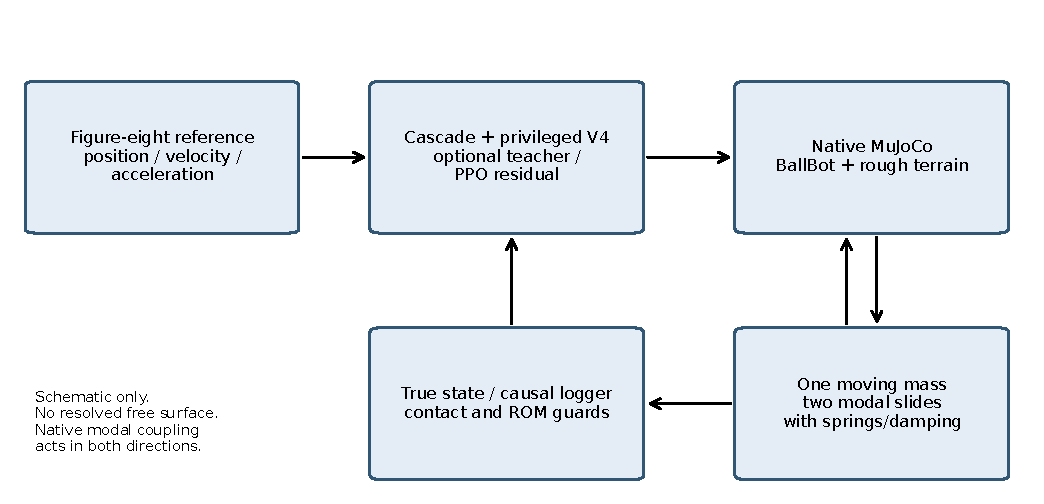
\includegraphics[width=.9\textwidth]{figures/fig01.pdf}\caption{Source-based architecture, explicitly schematic. Two-way arrows concern the native modal mechanical plant, not a resolved fluid surface.}\end{figure*}
